\documentclass[11pt,a4paper]{article}
\usepackage[utf8]{inputenc}
\usepackage[spanish,es-tabla]{babel}
\usepackage{graphicx}
\usepackage{fancyhdr}
\usepackage{float}
\usepackage[headheight = 110pt]{geometry}

\geometry{
	a4paper,
	left=30mm,
	right=30mm,
	top=20mm,
	bottom=20mm,
}

\newcommand{\codigoMateria}{86.06 }
\newcommand{\nombreMateria}{Circuitos Electrónicos}
\newcommand{\nroTP}{3}
\newcommand{\tipoInforme}{Preinforme}

\newcommand{\nombreDos}{Liaudat, Tobias}
\newcommand{\padronDos}{95540}

\newcommand{\nombreUno}{Gomez Peter, Federico}
\newcommand{\padronUno}{96091}

\begin{document}

\begin{center}
	\textbf{Universidad de Buenos Aires\\
	Facultad de Ingeniería}\\
	\vspace{1em}
	\begin{center}
		
\includegraphics{../img/fiuba.jpg}
	\end{center}
	\LARGE{\codigoMateria - \nombreMateria\\
	Trabajo de Laboratorio n$^\circ$\nroTP\\}
	\vspace{1em}
	\large{\tipoInforme}
\end{center}

\nombreUno - \#\padronUno 

\nombreDos - \#\padronDos 

\begin{abstract}
	En el presente informe se analizará la respuesta en frecuencia de una etapa amplificadora formada por dos transistores integrados de tecnología metal-óxido-semiconductor, de canal preformado, en configuracion cascode.
\end{abstract}

\newpage
%%%%%%%%%%%%%%%%%%%%%%%%%%%%%%%%%%%%%%%%%%%%%%%%%%%%%%%%%
%cabecera de las paginas

\pagestyle{fancy} % seleccionamos un estilo
\fancyhead{}
\fancyfoot{}
\lhead{
\includegraphics[width= 2.5 cm]{../img/logofiuba}} 
\rhead{\nombreMateria \, (\codigoMateria)} % texto centro de la cabecera
\cfoot{\thepage}

\newcommand{\HRule}{\rule{\linewidth}{100mm}} %linea negra de separacion
\raggedbottom %evita espacios en blancos grandes entre imagenes y textos
%%%%%%%%%%%%%%%%%%%%%%%%%%%%%%%%%%%%%%%%%%%%%%%%%%%%%%%%%


%	Conductancia
\newcommand{\mS}{\mbox{mS}}

%	Tensiones

\newcommand{\V}{\mbox{V}}
\newcommand{\mV}{\mbox{mV}}

%	Corrientes

\newcommand{\A}{\mbox{A}}
\newcommand{\mA}{\mbox{mA}}
\newcommand{\uA}{\mu \mbox{A}}
\newcommand{\nA}{\mbox{nA}}

%	Resistencias
\newcommand{\ohm}{\Omega}
\newcommand{\Kohm}{\mbox{K}\Omega}
\newcommand{\Mohm}{\mbox{M}\Omega}

%	Capacitores
\newcommand{\F}{\mbox{F}}
\newcommand{\mF}{\mbox{mF}}
\newcommand{\uF}{\mu \mbox{F}}
\newcommand{\nF}{\mbox{nF}}
\newcommand{\pF}{\mbox{pF}}

%	Frecuencias
\newcommand{\Hz}{\mbox{Hz}}
\newcommand{\KHz}{\mbox{KHz}}
\newcommand{\MHz}{\mbox{MHz}}
\newcommand{\GHz}{\mbox{GHz}}

%	TBJ
\newcommand{\VBE}{\mbox{V_{BE}}}
\newcommand{\vBE}{\mbox{v}_{BE}}
\newcommand{\vbe}{v_{be}}

\newcommand{\VCE}{\mbox{V}_{CE}}
\newcommand{\VCEQ}{\mbox{V}_{CEQ}}
\newcommand{\vCE}{\mbox{v}_{CE}}
\newcommand{\vce}{v_{ce}}

\newcommand{\IC}{\mbox{I}_{C}}
\newcommand{\ICQ}{\mbox{I}_{CQ}}
\newcommand{\iC}{\mbox{i}_{C}}
\newcommand{\ic}{i_{c}}

\newcommand{\IBQ}{\mbox{I}_{BQ}}
\newcommand{\iB}{\mbox{i}_{B}}
\newcommand{\ib}{i_{b}}

%	Mosfet
\newcommand{\VT}{\mbox{V}_T}

\newcommand{\VG}{\mbox{V}_{G}}
\newcommand{\VD}{\mbox{V}_{D}}
\newcommand{\VS}{\mbox{V}_{S}}

\newcommand{\VGS}{\mbox{V}_{GS}}
\newcommand{\VGSQ}{\mbox{V}_{GSQ}}
\newcommand{\VGSQuno}{\mbox{V}_{GSQ1}}
\newcommand{\VGSQdos}{\mbox{V}_{GSQ2}}
\newcommand{\vgs}{\mbox{v}_{gs}}
\newcommand{\vGS}{\mbox{v}_{GS}}

\newcommand{\VDS}{\mbox{V}_{DS}}
\newcommand{\VDSQ}{\mbox{V}_{DSQ}}
\newcommand{\vDS}{\mbox{v}_{DS}}
\newcommand{\vds}{v_{ds}}

\newcommand{\IDQuno}{\mbox{I}_{DQ1}}
\newcommand{\IDQdos}{\mbox{I}_{DQ2}}
\newcommand{\IDQ}{\mbox{I}_{DQ}}
\newcommand{\iD}{\mbox{i}_{D}}
\newcommand{\ID}{\mbox{I}_{D}}
\newcommand{\id}{i_{d}}

\newcommand{\iG}{\mbox{i}_{G}}
\newcommand{\ig}{i_{g}}

\newcommand{\rgs}{\mbox{r}_{gs}}
%	Jfet

\newcommand{\hFET}{\beta_{FET}}

\newcommand{\VP}{\mbox{V}_P}

\newcommand{\IDss}{\mbox{I}_{Dss}}


%	Pequeña señal
\newcommand{\rpi}{\mbox{r}_\pi}
\newcommand{\rmu}{\mbox{r}_\mu}
\newcommand{\ro}{\mbox{r}_o}
\newcommand{\gm}{\mbox{g}_m}
\newcommand{\gmuno}{\mbox{g}_{m1}}
\newcommand{\gmdos}{\mbox{g}_{m2}}

%	Parametros Transistores general
\newcommand{\Ri}{\mbox{R}_{i}}
\newcommand{\Riuno}{\mbox{R}_{i1}}
\newcommand{\Ridos}{\mbox{R}_{i2}}
\newcommand{\RiG}{\mbox{R}_{iG}}
\newcommand{\Ro}{\mbox{R}_o}

\newcommand{\RS}{\mbox{R}_S}


\section{Desarrollo}
Comenzando con el informe, se conecta el integrado de doble gate, BF966, en configuracion cascode (source común, gate común). El diagrama del circuito utilizado puede verse en la figura \ref{im:circuito}.

\begin{figure}[ht]
	\centering
	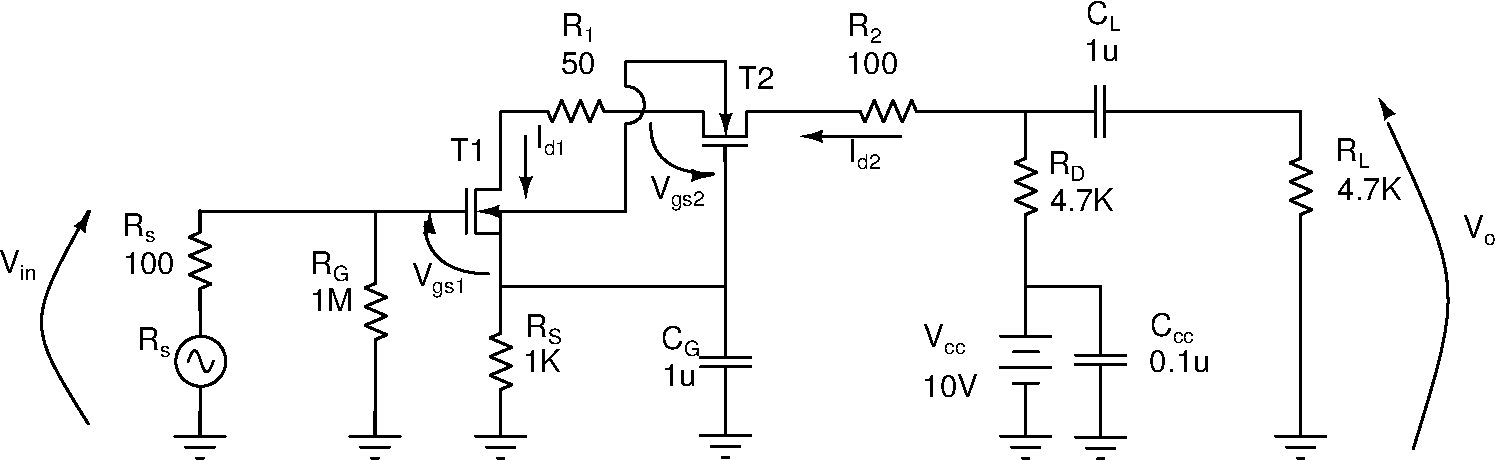
\includegraphics[scale=0.5]{../img/circuitoTL3.pdf}
	\caption{Conexión del circuito a analizar}
	\label{im:circuito}
\end{figure}

Para simplificar el analisis, se admiten por despreciable los parametros $\lambda = 0$ y $\gamma = 0$. De esta forma, no habrá variación de los $V_T$ de cada uno a causa del cortocircuito de los substratos. Viendo la hoja de datos del circuito, se extrajeron los siguientes valores de capacitancias parasitas, que pueden verse en la tabla \ref{ta:capacitanciasParasitas}.

\begin{table}[ht]
\begin{center}
\begin{tabular}{|c|c|c|c|}
\hline 
$C_{issg1}$ & $C_{issg2}$ & $C_{rss}$ & $C_{oss}$ \\ 
\hline 
$2.2\pF$ & $1.1\pF$ & $25\pF$ & $0.8\pF$ \\ 
\hline 
\end{tabular}
\end{center} 
\caption{Valores de capacitancias parasitas del integrado BF966}
\label{ta:capacitanciasParasitas}
\end{table}

El modelo simplificado de la estructura interna del integrado puede verse en la figura \ref{im:modeloIntegrado}.

\begin{figure}[ht]
	\centering 
	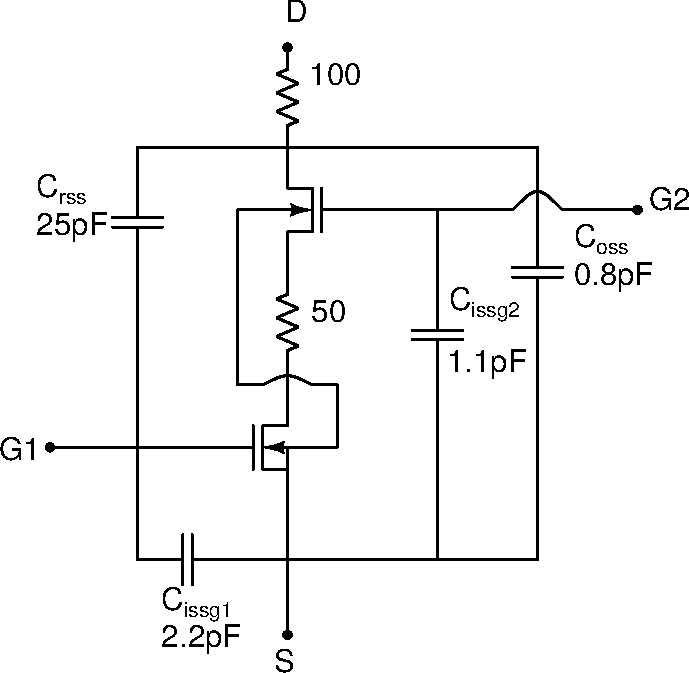
\includegraphics[scale=0.7]{../img/integrados.pdf}
	\caption{Modelo del circuito integrado}
	\label{im:modeloIntegrado}
\end{figure}

Los parametros característicos de ambos transisores pueden verse en la tabla \ref{ta:parametrosTransistor}.

\begin{table}[ht]
\begin{center}
\begin{tabular}{|c|c|c|c|}
\hline 
 & kp & $\VT$ & $\frac{W}{L}$ \\ 
\hline 
T1 & $15\frac{\mA}{\V^2}$ & $-1\V$ & $1$ \\ 
\hline
T2 &  $200\frac{\mA}{\V^2}$  & $-1\V$ & $1$\\
\hline
\end{tabular} 
\end{center}
\end{table}

Se procederá a analizar en primera instancia los valores del reposo del circuito de la figura \ref{im:circuito}. Luego se analizará la amplficación en frecuencias, para finalmente determinar la respuesta de este en bajas y altas frecuencias. Todo esto se hará primero de forma teórica, para luego ser contrastada mediante simulación y por medio de mediciones.

\section{Polarizacion}
\subsection{Cálculo Teórico}

El circuito de polarización puede observarse en la figura \ref{im:polarizacion}. Como puede verse, el gate del transistor 1 se encuentra a una tensión de $0\V$. Con este dato, y recorriendo la malla de transferencia, reempĺazando la corriente de drain por la ecuación característica del MOSFET se obtiene la siguiente ecuación:

\begin{equation}
	\VGSQuno = 0 - \IDQuno * 1\Kohm
\end{equation}

\begin{equation}
	\frac{\VGSQuno}{1\Kohm} = -\frac{\mbox{kp}}{2} \cdot (\VGSQuno - \VT)^2
	\label{eq:VGSQ1}
\end{equation}

Reemplazando los datos conocidos en \ref{eq:VGSQ1} se obtiene un $\VGSQuno = -0.7\V$. Para obtener $\VGSQdos$ se parte conociendo la tensión contra común del gate del transistor 2. Mediante un calculo similar, se obtiene un $\VGSQdos = -0.916\V$. Las tensiones contra comun y la corriente de polarización pueden verse en la tabla \ref{ta:datosPolarizacion}.

\begin{table}[ht]
	\begin{center}
		\begin{tabular}{|c|c|c|c|c|c|}
		\hline 
		 & $\VS$ & $\VG$ & $\VD$ & $\IDQ$ & $g_m$ \\ 
		\hline 
		T1 & $0.7\V$ & $0\V$ & $1.616\V$ & $0.7\mA$ & $4.5\mS$ \\ 
		\hline 
		T2 & $1.616\V$ & $0.7\V$ & $6.71\V$ & $0.7\mA$ & $16.8\mS$ \\ 
		\hline 
		\end{tabular} 
	\end{center}
	\caption{Valores de polarización del circuito amplificador calculados teóricamente}
	\label{ta:datosPolarizacion}
\end{table}


\subsection{Simulación}

Luego se prosigue a simular el circuito y ver su polarización. Se simulo el circuito de la figura \ref{im:circuito} utilizando el programa \textsl{LTSpice}.Los valores obtenidos se pueden ver en la tabla  \ref{ta:datosPolarizacion_sim}. 


\begin{table}[ht]
	\begin{center}
		\begin{tabular}{|c|c|c|c|c|c|}
		\hline 
		 & $\VS$ & $\VG$ & $\VD$ & $\IDQ$ & $g_m$ \\ 
		\hline 
		T1 & $0.695\V$ & $0\V$ & $1.612\V$ & $0.695\mA$ & $4.57\mS$ \\ 
		\hline 
		T2 & $1.612\V$ & $0.695\V$ & $6.662\V$ & $0.695\mA$ & $16.7\mS$ \\ 
		\hline 
		\end{tabular} 
	\end{center}
	\caption{Valores de polarización del circuito amplificador obtenidos mediante simulación}
	\label{ta:datosPolarizacion_sim}
\end{table}

Se puede observar que los valores obtenidos en el simulación coinciden con los obtenidos teóricamente. Esto confirma que las aproximaciones realizadas fueron válidas.



\section{Análisis a frecuencias medias}
\subsection{Cálculo teórico}

Para dichas frecuencias, se consideran los capacitores externos como cables (poseen una impedancia tan chica que se puede despreciar su efecto en estas frecuencias), mientras que las parásitas del integrado se consideran como abiertos. El esquema para este análisis puede verse en la figura \ref{im:frecuenciasMedias}.

\begin{figure}[ht]
	\centering
	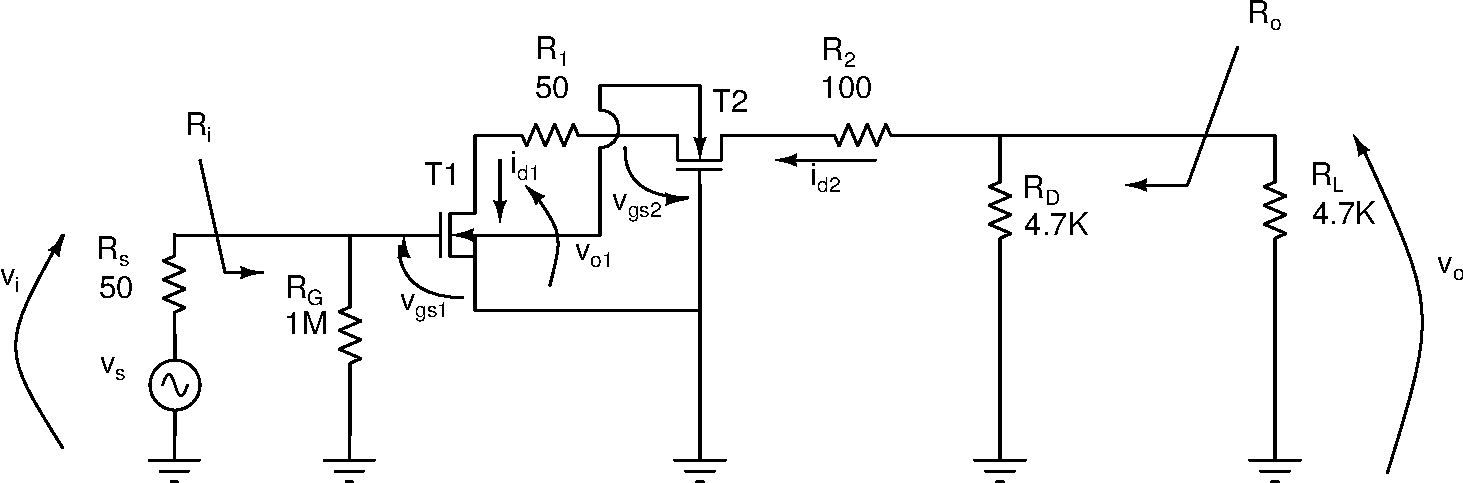
\includegraphics[scale=0.5]{../img/frecuenciasMedias.pdf}
	\caption{circuito amplificador a frecuencias medias.}
	\label{im:frecuenciasMedias}
\end{figure}

Con estos sentidos de referencias se procederá a calcular los parámetros de amplificación, además de obtener los valores de resistencias de entrada y salida.

La expresión de la ganancia de la etapa emisor común puede verse en la siguiente ecuación:

\begin{equation}
	A_{v1} = \frac{v_{o1}}{v_i} = \frac{-\id \cdot (50 +\Ridos)}{\vgs}
\end{equation}

La resistencia de entrada del transitor dos, $\Ridos$ vale:
\begin{equation}
	\Ridos = \frac{\rpi}{\hFET} = \frac{1}{\gmdos}
	\label{eq:Ri2}
\end{equation}

La ganancia del primer transistor entonces es de:

\begin{equation}
	A_{v1} =-\gmuno(\frac{1}{\gmdos}+50\ohm) = -0.5
	\label{eq:Av1}
\end{equation}

Esta ganancia, si bien es muy baja considerando que es un transistor en emisor común, resulta lógico, ya que como carga se está conectando un transitor base común, cuya característica principal es una resistencia de entrada muy baja. Para el transistor 2, se procede de la misma forma que con el transistor 1:

\begin{equation}
	A_{v2} = \frac{v_o}{v_{o1}} = \frac{- \id \cdot \mbox{R}_{ca}}{- \vgs - \id 50\ohm} = \frac{1}{\frac{1}{\gmdos}+50\ohm} \cdot 2.35\Kohm = 21.46
	\label{eq:Av2}
\end{equation}

La ganancia total del circuito es de $-10.73$.

Por inspección, los valores de la resistencias de entrada y de salida de todo el bloque son los siguientes:

\begin{equation}
	\Ri = 1\Mohm // \rgs = 1\Mohm 
\end{equation}

\begin{equation}
	\Ro = 4.5\Kohm // R_{oc} = 4.7\Kohm
\end{equation}

\begin{equation}
	R_{oc} = \ro \cdot (1 + \frac{\hFET \cdot R_s}{\rgs}) \rightarrow \infty
\end{equation}

Estos valores son los ideales. Cuando se simule, y sobre todo cuando se realicen las mediciones, los valores de las resistencias tenderán a cambiar, sobre todo la de entrada. Esto se debe a la influencia que tendrá el equivalente de la punta de osciloscopio.

Con estos valores calculados, se procederá a medir las máximas excursiones sin recorte. Para comenzar con esto, se admite que la entrada $\hat{\V}_{imax}$ es tal que no distorsiona por alinealidad. Para lograr esto, la señal de entrada debe cumplir:

\begin{equation}
	\hat{\V}_{ime sin distorosion} < \frac{\VGSQ - \VT}{2}
	\label{eq:viSinDistorsion}
\end{equation}

Para llegar a esta ecuación se debe partir de que la ecuación de la corriente de drain, aproximarla a una recta y buscar la ordenada al origen de esta recta, como se puede ver en la figura \ref{im:maximaExcursionSinDistorsion}.

\begin{figure}
	\centering
	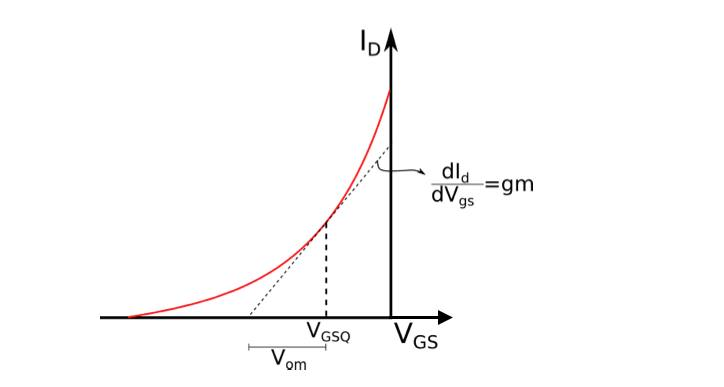
\includegraphics[scale=0.5]{../img/distorsion.jpg}
	\caption{Esquema de corriente de drain en función de la tension gate-source de un MOSFET de canal preformado}
	\label{im:maximaExcursionSinDistorsion}
\end{figure}

\begin{eqnarray}
		v_{om} = \vGS - v_{om_0} \\
		v_{om} = \VGSQ - v_{om_0} \\
		v_{om_0}= \VGSQ - \frac{\IDQ}{\gm} \\
		v_{om} = \frac{\IDQ}{\gm} \\
		v_{om} = \frac{\VGSQ - \VT}{2}
\end{eqnarray}

Para el primer transistor se debe cumplir que $\vGS < 0.155\V$, mientras que para el segundo $\vGS < 0.042\V$. Para que el segundo transistor vea una $\vGS = 0.042\V$, se debe tener un $v_i = \frac{0.042}{|A_{v2}|} = 0.084\V$. Por lo tanto, la tension de alimentanción $v_s \ll 0.084\V$.  

\end{document}